% Use only LaTeX2e, calling the article.cls class and 12-point type.

\documentclass[12pt]{article}

\usepackage{times}

% Packages I manually added
\usepackage{graphicx}
\usepackage{placeins}
\usepackage{float}
\usepackage{amsmath}
\usepackage{hyperref}

\topmargin 0.0cm
\oddsidemargin 0.2cm
\textwidth 16cm
\textheight 21cm
\footskip 1.0cm


\title{Well-Designed Environmental Markets Enable Large-Scale Marine Conservation}


% Place the author information here.  Please hand-code the contact
% information and notecalls; do *not* use \footnote commands.  Let the
% author contact information appear immediately below the author names
% as shown.  We would also prefer that you don't change the type-size
% settings shown here.

\author{Juan Carlos Villase\~{n}or-Derbez,$^{1\ast}$ John Lynham,$^{2}$ Christopher Costello$^{1}$\\
\\
\normalsize{$^{1}$Bren School of Environmental Science \& Management,}\\
\normalsize{University of California at Santa Barbara, Santa Barbara, CA}\\
\normalsize{$^{2}$Department of Economics, University of Hawaii at Manoa, Honolulu, HI}\\
\\
\normalsize{$^\ast$To whom correspondence should be addressed; E-mail: juancarlos@ucsb.edu.}
}

% Include the date command, but leave its argument blank.

\date{}



%%%%%%%%%%%%%%%%% END OF PREAMBLE %%%%%%%%%%%%%%%%



\begin{document}

% Double-space the manuscript.

\baselineskip24pt

% Make the title.

\maketitle



% Place your abstract within the special {sciabstract} environment.
\begin{abstract}
While it is commonly agreed that marine conservation should expand dramatically around the world, most countries have yet to implement large-scale Marine Protected Areas in their own waters. When a country closes a large fraction of its waters to fishing, it stands to lose significant fishery revenue. While this may be more-than-made-up-for through spillover, these benefits typically accrue to other countries or the high seas. We show that careful design of cross-country rights-based approaches to fisheries can actually incentivize, rather than relegate, large scale marine conservation. By combining a model of cross-country trading of rights with vessel-level tracking data before and after a large-scale conservation action is implemented, we show that two market design features are pivotal to encouraging such conservation. First, only when trading of fishing rights across countries is allowed, can a conservation-minded country capture the economic spillover benefits of their conservation actions. Second, the allocation of rights to countries must not be watered-down over time by a country's conservation efforts; for example, a country's annual allocation of rights should depend on the size of the fish stock in their waters, not on how hard it has fished. Overall, these results provide a template for how to incentivize countries to engage in large-scale marine conservation within a market-based setting.
\end{abstract}

\clearpage

\section{Main}

Recognizing the need to protect marine biodiversity and ecosystem services, various international bodies have committed to dramatically expand marine protection around the world by protecting 30\% of the oceans \cite{oleary_2016,dinerstein_2019}, and that large portions of these will be entirely no-take \cite{sala_2017,sala_2018}. While most marine protected areas (MPAs) implemented to date have been small, it is widely-recognized that to meet these goals, very large MPAs must also be part of the strategy. But would any country rationally close 30\%, 80\% or even 100\% of its waters to fishing if this means losing all fishing revenue from within the closed area? At first glance, the answer is probably ``no''. Losing this important source of revenue would cripple many fishing-dependent economies, particularly the Pacific Island nations who are viewed as viable candidates for large closures \cite{mcleod_2019}. On the other hand, the closure may generate substantial ``spillover'' of larvae and adult fish \cite{ramesh_2019,hernndez_2019} and other benefits into adjacent waters which could, in principle, offset these losses. The problem with this argument is that for very large MPAs, these spillover benefits could accrue to other nations and the high seas \cite{agardy_2018}, with no obvious mechanism for the conserving country to recoup them. A viable solution may lie in international fishing effort markets, where nations trade the right to fish with each other. The design and effectivness of fishing effort markets for fisheries management have been explored before \cite{havice_2010,havice_2013}, but little attention has been given to the role that markets can play in conservation. Here, we will show how fishing effort markets can be designed (if new) or modified (if already existing) to incentivize implementation of large-scale marine protected areas.

We are motivated by a real-world but relatively understudied institution called the Parties to the Nauru Agreement (PNA). The PNA is a coalition of nine Pacific island nations that collectively manages tuna purse seine fishing in its members' waters (Fig. \ref{fig:PNA_map}) \cite{havice_2013,aqorau_2018}. These waters account for 14.5 million km\textsuperscript{2} (an area four times larger than the continental US), and over 60\% of skipjack tuna catch in the Western Central Pacific \cite{havice_2013}. The PNA manages this tuna purse seine fishery using a vessel-day scheme (VDS) where total annual fishing effort is capped at around 45,000 vessel-days. Vessel-days are allocated across the nine nations, which then lease them to fishing vessels. A vessel-day grants a fishing vessel the right to fish for 24 hours within one of the nine Exclusive Economic Zones (EEZs) within the PNA. Member nations derive enormous benefits from leasing these fishing rights to foreign fleets, in some cases exceeding half of a country's GDP. In addition to highly productive tuna fisheries, the PNA waters provide a wealth of ecosystem benefits, hence the focus on large-scale conservation efforts in the region \cite{mcleod_2019}. In 2015, Kiribati, a PNA member, created the Phoenix Islands Protected Area, one of the largest protected areas on earth (408,250 km\textsuperscript{2}), and Palau will close 80\% of its national waters to fishing by December 2020. We draw from the PNA's market-based approach to managing tuna fisheries and build on it to show how the market can be designed to incentivize conservation.

Not all market-based approaches to environmental management are created equal. A pervasive finding across a range of natural resources is that features of markets, such as the allocation of rights, can have implications for the market's functioning \cite{libecap_1989}. In the context of fishing effort markets, we find that two market design features are pivotal in determining the incentives for large-scale marine conservation: trading and allocation rules. But why would these design features of a fisheries market affect the incentives for conservation? Consider the incentives for a country to close 100\% of its waters. Such a closure would surely benefit other countries through the spillover of fish from the protected area to the waters of neighboring countries. If the conserving country could trade the rights to catch the fish that spillover, other countries would likely buy them, offsetting the costs of not fishing its own waters. But if the conserving country was not allowed to lease these rights, then it would lose all of its fishing revenue. The rules for how fishing rights are allocated across countries are equally important. Suppose rights are allocated each year based on the previous year's fishing effort: the more a country fishes, the more it gets allocated the next year. This would clearly disadvantage a conservation-minded country and, in fact, might reward undesirable behavior. In the following section, we will show how trading and allocation rules can shape the incentives that may facilitate or hinder large-scale conservation. We will then make use of vessel-tracking data to analyze a real-world case of large-scale marine conservation under fishing effort markets.

\subsection{Designing markets for conservation}

To examine how market design incentivizes or punishes large-scale conservation, we develop a 10-country spatial bioeconomic model that mirrors the strategies and spatial connections among the nine PNA nations and the high seas. Countries 1 to 9 represent the PNA countries, which operate under a vessel-day scheme where vessel-days are capped for each country and closely tracked. ``Country'' 10 represents the high seas, where fishing days are unregulated and determined by prevailing economic conditions. We examine the effects of large-scale conservation in a single country (Country 1) under markets with and without trading between countries. In all cases, we solve the bioeconomic model for the equilibrium vessel-day price, fishing effort redistribution, and fish stock that would be expected to occur in the market. We quantify the change in revenue to Country 1 and compare each scenario to a benchmark scenario without any conservation action. We simulate these outcomes across a range of reserve sizes and assumptions about within-country stock movement (see the Methods section for details).

We first simulate a fishery where trading between countries is not allowed. This represents the status quo of any nation unilaterally engaging in large-scale conservation. Intuitively, we find that a spatial closure in Country 1 will always result in a loss in revenues to Country 1 (Fig. \ref{fig:PNA_model}A). Higher within-country stock movement ($\theta$ = 0 implies no within-country movement and $\theta = 1$ implies that fish are well-mixed within the fishing season) allows vessels to harvest the stock within the remaining open area, lowering the cost to Country 1. The closure-to-cost ratio for any reserve size is greater than 1:1 when stock movement is low (\emph{i.e.} $\theta < 0.2$), implying that a 30\% closure would result in at least a 30\% loss in revenues. Even for a highly mobile stock where fish can move in and out of the reserve, a spatial closure reduces the amount of biomass that is available for harvest in the conserving country (\emph{i.e.} biomass outside the reserve), which reduces vessels' willingness to pay to fish in such waters (Fig. S1). When countries cannot trade, the costs of conservation are incurred by Country 1, but the benefits are received by the eight other countries (revenues increase between 0\% and 6\% each; Fig. S2) and the high seas. This benchmark simulation highlights the misalignment of incentives, where a conservation-minded country incurs large costs and provides public benefits to other nations with no mechanism for recouping these benefits.

How would trading between countries change these results? We simulate the same fishery, but now allow for vessel-days to be traded across countries (as is the case for the PNA). As before, a closure in Country 1 lowers the value of vessel-days in that country (because the fishable water shrinks). But increased biomass in other countries causes their vessel day prices to increase. As a result, vessel-days from Country 1 are traded to Countries 2 to 9, until prices equalize across countries (Fig. S3). Under this market design, revenue losses are less than 1\%, compared to the base case with no reserve (Fig. \ref{fig:PNA_model}B; note that the vertical axis now only ranges from 0 to 0.8\% instead of from 0 to 100\% as in Fig. \ref{fig:PNA_model}A). With trading, the relative revenue drop will always be smaller than the relative effort drop, and the opposite is observed when there is no trading (Fig. S4). Overall, this shows that 88\% to 99\% of the costs of conservation can be avoided if markets are designed to allow trading (Fig. \ref{fig:PNA_model}C).

We have shown that trading significantly reduces the costs of conservation. However, a new question arises. How should rights be re-allocated every year once a country starts closing its waters to fishing? Customarily, the allocation of fishing effort rights is a formula that combines historical fishing effort and biomass in a country's waters \cite{havice_2013}. We test a range of allocation rules that weigh effort ($\alpha$) and biomass ($1 - \alpha$) differently as the basis for ongoing rights allocation. We simulate a fishery operating with closures for 50 years and compare the resulting revenues to a fishery without any closures. We find that when allocation is based on historical effort only (\emph{i.e.} $\alpha = 1$), implementing a reserve results in long-term losses to the conserving country of 20\% to 93\%, depending on the size of reserve and stock movement (Fig. \ref{fig:allocation_cost_plot}). However, a biomass-only allocation rule (\emph{i.e.} $\alpha = 0$) results in revenue losses as low as 0.1\% to 0.7\%, essentially eliminating the costs of conservation. This result implies that if allocation is based purely on the biological features of a stock (\emph{e.g.} the biomass within a nation's waters), and not on fishing effort, the incentives for conservation are sustained through time.

\subsection{Markets and conservation in practice}

A large-scale MPA was recently implemented in PNA waters, providing the ideal empirical setting to test our predictions. In January 2015, Kiribati closed 11.5\% of its EEZ to implement the Phoenix Island Protected Area (PIPA), effectively displacing all fishing effort within its boundaries\cite{mccauley_2016,mcdermott_2018}. By protecting important tuna spawning habitat, PIPA may provide important recruitment and biomass benefits to adjacent waters \cite{hernndez_2019}. We combine vessel-tracking data \cite{kroodsma_2018} and country-level license revenue data reported by the Pacific Islands Forum Fisheries Agency (FFA) \cite{ffa_2017} to quantify the displacement of vessel-days and the likely costs of conservation. Of the 318 tuna purse seine vessels that fished in PNA waters between 2012 and 2018, 64 ``displaced'' vessels fished within PIPA at least once prior to its implementation and 254 ``non-displaced vessels'' never fished in PIPA waters but fished within the PNA waters. We use the tracking data to calculate vessel-days in the same way that the PNA does (see Methods for details) and the redistribution of fishing events before and after the implementation of PIPA.

Consistent with our models' prediction, after PIPA was implemented, displaced vessels relocated largely outside of Kiribati, and into other PNA countries' waters (Fig \ref{fig:fishing_raster_diff} and Figs. S6). Indeed, from 2014 to 2015, displaced vessels spent 2,115 fewer vessel-days (a 25\% reduction) in Kiribati, and 2,298 fewer vessel-days in PNA waters (a 17 \% reduction; Fig. \ref{fig:empirical}). On the other hand, non-displaced vessels spent 4,656 additional days in Kiribati during 2015, and an additional 9,598 vessel-days in PNA waters. By 2018, we observe a net decrease of vessel-days within Kiribati, from 12,671 in 2014 to just 7,677 in 2018, with displaced vessels driving the decrease (Fig. \ref{fig:empirical}A). However, aggregate effort at the PNA-level remains relatively constant and we do not observe a ``fishing the line'' effect (Fig S7). The reduction in effort to Kiribati and constant effort at the PNA-level suggest that trading facilitated redistribution of effort within PNA waters, just as the model predicted.

The decrease of vessel-days in Kiribati could be alternatively (or jointly) explained by changes in oceanographic conditions that drive distribution of target species and fishing vessels. For example, as El Niño events develop, tuna species are known to shift longitudinally across PNA waters, causing vessels to redistribute \cite{aqorau_2018,hanich2018unraveling}. However, the total decrease that we observe for Kiribati in Fig. \ref{fig:empirical} is driven by the relocation of vessels that once fished within PIPA, not the entire fleet. One could argue that differences in vessel characteristics between displaced and non-displaced vessels may influence their ability to redistribute or take advantage of different oceanographic conditions in Kiribati. For example, on average, displaced vessels have smaller crew sizes, more engine power, and are larger than non-displaced vessels (Table S2, Fig. S5). However, displaced vessels gradually reduce their time spent in PNA waters too.

As predicted by our theoretical model, the implementation of PIPA resulted in a decrease in fishing effort within Kiribati's water without large revenue losses. Kiribati's reported revenue increased from US\$127.3 million in 2014 to US\$148.8 million in 2015, before decreasing to US\$118.3 million in 2016 (Fig. \ref{fig:empirical}C). The increase and subsequent decrease in revenues matches the vessel-day patterns observed for Kiribati from 2014 to 2016 (Fig. \ref{fig:empirical}D). But, critically, the drop in revenue in 2016 (20\%) is smaller than the drop in VDS effort (35\%). This supports a key prediction of our model: with trading, the relative revenue drop will always be smaller than the relative effort drop but, without trading, the opposite relationship would hold (Fig. S4). At the PNA level, total revenues showed a net increase of \$64.7 and \$28 million USD for 2015 and 2016 respectively (Fig. S8), despite the PIPA closure.

Our findings may help inform management and implementation of existing and upcoming MPAs in the PNA. In January 2020, Palau will close nearly 80\% of its EEZ to commercial fishing to create the Palau National Marine Sanctuary (PNMS): the 14\textsuperscript{th} largest protected area in the world (Fig. \ref{fig:PNA_map}). Vessel-tracking data (2012 to 2018) shows that the proposed PNMS boundaries contain 65.6 $\pm$ 0.08\% ($\pm$ 1SD) of longline vessel-days (non-tradable) and 82.2 $\pm$ 0.08\% ($\pm$ 1SD) of purse seine vessel-days (tradable; Fig. S10-S11).

%%%% PLEASE TAKE A LOOK AT THE SECOND SENTENCE OF THIS PARAGRAPH %%%%
While trading would allow Palau, Kiribati, and other PNA members to reduce revenue losses from large-scale conservation, our model indicates that moving from a 40\% biomass-based allocation rule to a 100\% biomass-based rule would ensure long-term financial security in the presence of large-scale MPAs, and further incentivize conservation within the PNA. However, it is worth mentioning that we did not empirically test this prediction, as this would imply modifying the allocation rule in the real world. The Parties to the Nauru Agreement have shown that rights-based management of transboundary resources can result in large management and economic benefits \cite{havice_2013,aqorau_2018}. By facilitating trade and allocating rights based on biomass, they may become pioneers in effective large-scale marine conservation in a market-based setting.

There are, however, a series of important considerations to take into account. Firstly, in our study only one of the countries considers the implementation of a protected area. However, an interesting extension would be that of cooperative conservation. In that setting, a group of countries could coordinate on an optimized, large-scale strategic closure -perhaps using vessel-day trading as a means of compensation- in a manner similar to the model above. Future research could explore the role of heterogeneous costs and benefits between countries, and the way in which these can shape conservation outcomes in a market-based setting. A second consideration is that of the role that the high seas play: environmental markets require secure property rights, which are lacking in the high seas \cite{crespo_2019}. Any spillover from into the high seas could potentially be eroded by the prevailing open access conditions. Therefore, a conservation-minded nation has no mechanism to capture the benefits provided to the high seas, highligting the importance of empowering high seas governance and transboundary cooperation \cite{aqorau_2018,crespo_2019}.

The use of environmental markets for conservation is a common but contentious approach among conservation scientists and resource managers \cite{sandbrook_2019}. One of the driving concerns is that markets may create incentives that lead to undesirable outcomes, thus emphasizing the need for careful design. We show that individual countries have little incentive to undertake large-scale marine conservation, but that this incentive can be reversed if those countries are in an appropriately-designed market-based setting. For the market to create these incentives, certain design features are paramount. In the case of fishing rights and MPAs, cross-country transferable fishing rights and a biomass-based allocation rule are two necessary conditions to achieve the conservation incentive. International goals over the next decade have set ambitious targets for terrestrial and marine conservation, which will provide benefits ranging from preserving biodiversity to enhancing human well-being \cite{oleary_2016,dinerstein_2019,roberts_2017,ban_2019}. Our work shows how well-designed environmental markets can provide the right incentives for effective large-scale marine conservation.

\clearpage

\section{Methods}

\subsection{Bioeconomic model}

We model a 10 country discrete-time meta-population system, where Country 1 considers a spatial closure. Countries 1 - 9 operate under a vessel-day scheme, and Country 10 represents the high seas and other areas not managed under a VDS. The stock of fish in each country is relatively stationary within a single fishing season, but  growth from escapement redistributes across all countries annually. The price of fish is $p$, and catchability is given by $q$. These parameters are held constant across countries.

\subsubsection{Fishery dynamics}

In the absence of a reserve, the revenue for vessels in country $i$ is given by $pqE_iX_i$, where $E_i$ and $X_i$ are effort (vessel-days) and stock size in country $i$ at the beginning of a period. The cost of fishing in country $i$ is given by $cE_i^\beta$, where $\beta = 1.3$ matches commonly-used cost functions that assume increasing units of effort are increasingly costly to apply \cite{costello_2016}.

Country 1 considers a spatial closure by implementing a reserve as a fraction $R$ of the total country ($R \in[0,1)$). Fish move within a country based on $\theta$, where $\theta = 0$ implies no movement within the country, and $\theta = 1$ implies that fish move so much that they can be caught from anywhere within the country (see the \emph{Notes on within-country fish movement} section below). In this country, revenues are given by $pqE_1X_1(\theta + (1 - \theta)(1 - R))$. The parameterization of movement and reserve size imply that profit from fishing Country 1 is given by:

$$
\Pi_1(E_1,X_1,R) = pqE_1X_1\Omega_1-cE_1^\beta
$$

\noindent with $\Omega_1 = (\theta + (1 - \theta)(1 - R))$ being a parameterization that combines reserve size as a proportion of country ($R =  [0, 1)$) and within-country fish movement ($\theta$). Under this parameterization, $\Omega_{i \neq 1} = 1$ since only Country 1 implements a reserve.

Therefore, we can generalize the country-level profit equation to:

$$
\Pi_i(E_i,X_i, R_i) = pqE_iX_i\Omega_i-cE_i^\beta
$$

\noindent The above equations imply that the marginal profit from the last unit of effort in a country are given by:

\begin{equation}
\pi_i(E_i) = \frac{\partial \Pi_i}{\partial E_i} = pqX_i\Omega_i - \beta cE_i^{\beta-1}
\label{eqn:marginal_profit}
\end{equation}

In practice, the effort levels in each country are allocated by management (so $E_{1},\ E_{2},...,E_{9}$ are given) and the effort level on the high seas ($E_{10}$) is a result of open access dynamics. Therefore, we assume that effort continues to enter Country 10 until the profit from the last unit of effort is exactly zero, indicating that $E_{10}$ is the value for which $\pi_{10}(E_{10})  = 0$. Setting Equation \ref{eqn:marginal_profit} for $i = 10$ equal to zero and removing $\Omega_{10} = 1$ for simplicity, we can solve for $E_{10}$:

\begin{equation}
E_{10} = \left(\frac{pqX_{10}}{\beta c}\right)^{\frac{1}{(\beta - 1)}}
\label{eqn:effort_hs}
\end{equation}

Under VDS-operated countries, however, profits from the marginal unit of effort should equate to the price of fishing in the country. Therefore vessel-day price for countries under VDS ($i = (1, 9)$) is  given by:

$$
\pi_i = pqX_i\Omega_i - \beta c E_i ^{\beta - 1}
$$

\noindent Solving for $E_i$ we obtain:

\begin{equation}
E_i = \left(\frac{pqX_i\Omega_i - \pi_i}{\beta c }\right) ^ {\frac{1}{\beta - 1}}
\label{eqn:demands}
\end{equation}

Equation \ref{eqn:demands} tells us the country-level effort for a given country-specific stock size ($X_i$) and vessel-day price ($\pi_i$). A vessel-day scheme establishes a cap on total effort allowed. This means that fishing effort from Countries 1 - 9 must add up to this limit (45,000 vessel-days). Therefore, total allowable effort in the fishery is given by:

\begin{equation}
\bar{E} = \sum_{i = 1}^9\left(\frac{pqX_i\Omega_i - \pi}{\beta c }\right) ^ {\frac{1}{\beta - 1}}
\label{eqn:Ebar}
\end{equation}

\noindent In the above Equation, vessel-day price is the same across all countries when trading is allowed; the subindex is dropped for this parameter.

\subsubsection{Stock dynamics}

Country-level harvest is then determined by effort and stock size:

\begin{equation}
H_i = qE_iX_i\Omega_i
\label{eqn:harvest}
\end{equation}


\noindent Therefore, escapement in country $i$ in time period $t$ is the difference between initial stock size and harvest given by $e_{i,t} = X_{i,t} - H_{i,t}$ and total escapement is $e_t=\sum_{i=1}^{10}e_{i,t}$. The entire stock then grows logistically according to:

\begin{equation}
X_{t+1} = e_t \times  e^{r \left(1 - \frac{e_t}{K} \right)}
\label{eqn:grow}
\end{equation}

\noindent where $r$ and $K$ are species-specific intrinsic growth rate and carrying capacity. After the stock grows, a constant and country-specific fraction $f_i$ of the total stock redistributes to country $i$, so:

\begin{equation}
X_{i,t+1} = f_iX_{t+1}
\label{eqn:disperse}
\end{equation}

\subsubsection{Vessel-day revenues}

The vessel-day price that a country charges is given by $\pi_i$ from Eqn \ref{eqn:marginal_profit}. Therefore, country-level license revenues are given by:

\begin{equation}
\omega_i = \pi_iE_i
\label{eqn:license_revenue}
\end{equation}

\noindent Equation \ref{eqn:harvest} shows that low values of $\theta$ and $R > 0$ would decrease harvest and increase escapement in Country 1, for a given level of effort and stock size. This would lead to an increase in total stock size (Equation \ref{eqn:grow}) and a benefit to all the other countries. But this would also cause the stock in the high seas ($X_{10}$) to increase, leading to increased effort being allocated to the high seas (Equation \ref{eqn:effort_hs}) and a loss of these potential rents. Thus, the spillover benefits of increasing $R$ are never completely captured. Information on model parameterization is provided in our Supplementary Materials.

\subsubsection{Notes on within-country fish movement}

In our model parameterization, the proportion of biomass ``available'' for harvest is given by  $\Omega_1 = (\theta + (1 - \theta)(1 - R))$. This implies that for a given country with stock size $X_i$, the total biomass available for harvest will be given by $\Omega X_i$. Consider the case of a sesile fish with $\theta = 0$. If the country were to close 50\% of its waters to fishing ($R = 0.5$), only 50\% of the stock would be available for harvest (\emph{i.e.} $0 + (1 - 0) * (1 - 0.5) = 0.5$). Now, consider the same closure is applied with a stock with high mobility, so $\theta = 0.9$. In this case, despite the closure, fish constantly swim between the reserve and fishing grounds making 95\% of biomass available for harvest (\emph{i.e.} $0.9 + (1 - 0.9) * (1 - 0.5) = 0.95$). As derived in the bioeconomic model above, a vessel's willingness to pay to fish in a given patch will be determined by the amount of biomass available for harvest. Within-patch stock movement therefore plays an important role in determinig a vessel's willingness to pay in the remaining open waters: a vessel will be willing to pay more to fish in waters where 95\% of biomass is available for harvest, than when only 50\% of biomass is available for harvest.

\subsubsection{Simulations}

We run simulations under two market designs and test the model across a range of reserve sizes and within-country movement parameters.The first scenario does not allow trading. In this case, total allowable effort ($\bar{E}$) and biomass $B_{now}$ are known and equally distributed among Countries 1-9. For Country 10, we solve for Eq \ref{eqn:effort_hs} until biomass converges to match $B_{now}$. We then proceed to ``close'' a portion of Country 1, and calculate the vessel-day price in Country 1 given that only $X_i\Omega_i$ biomass is available for harvest. We compare vessel-day revenues of each scenario to a case with no reserve ($R = 0$). This produces a measure of the cost of implementing a spatial closure of size $R$ in Country 1.

The second scenario allows trading. We start again by solving for the high seas to obtain total effort. Since a closure is not in effect and VDS-managed effort is equally distributed across the 9 countries, this equilibrium is the same as the first step above. We then implement a spatial closure in Country 1. This essentially lowers the price fishers would be willing to pay to fish in a country with only biomass $X_i\Omega_i$, lowering demand for vessel-days in Country 1. Countries 2 - 9 have a higher demand for vessel days, and therefore a portion of vessel-days from Country 1 are sold to Countries 2 - 9. This increases effort in these countries, which reduces escapement and therefore biomass. This reduction in biomass in turn will modify the marginal profit and willingness to pay to fish in each country. We therefore iterate this process until biomass stabilizes, finding the system's equilibrium. Like before, we calculate vessel-day revenues to each country and compare them to a case with no reserve in Country 1.

Annual vessel-days are often allocated based on a combination of historical within-country effort and biomass. In the PNA, 60\% of the allocation is calculated based on EEZ effort over the last seven years and 40\% is calculated based on the 10-year average of each country’s share of estimated biomass (of skipjack and yellowfin tuna) within its EEZ (This is explained in more detail in Article 12.5 of the 2012 Amendment to the Palau Agreement and in \cite{Hagrannsoknir2014}). Trading vessel-days to other countries would imply that historical within-country effort declines through time. The allocated days to a country with a full spatial closure would eventually be reduced to just the 40\% based on biomass.

In the trading scenario above, effort from Country 1 (with the reserve) is traded to other countries. This means that its allocation will decrease as purse seine effort in its EEZ is reduced. To analyze the consequences of different allocation rules when trading is allowed, we simulate a fishery 50 years into the future, and annually re-allocate vessel-days based on a 7-year running mean of country-level effort and biomass. At the end of every time period (a year), vessel-days are re-allocated to each country based on the following rule:

$$
E_{i,t+1}^* = \alpha
\left(\frac{\sum_{\tau = 0}^{\hat{\tau}}E_{i,t-\tau}}{\sum_{\tau = 0}^{\hat{\tau}}\bar{E}_{{t-\tau}}}
	\right)
	+
(1 - \alpha)
\left(\frac{\sum_{\tau = 0}^{\hat{\tau}}X_{i,t-\tau}}{\sum_{\tau = 0}^{\hat{\tau}}\bar{X}_{t-\tau}} \right)
$$

\noindent where $\alpha$ is a weight on historical effort ($E_i$) and $1-\alpha$ is the weight on historical biomass ($B_i$). We use $\hat{\tau}= 6$ to obtain a moving mean of 7 years for these measures. The difference between allocated days ($E_i^*$) and used days (determined by Equation \ref{eqn:demands}) for Country 1 are the sales. We then calculate vessel-day revenues to each country over the 50-year time horizon and compare to a case where there is no reserve and allocations are based solely on biomass ($\alpha = 0$).

\subsection{Empirical case study}

\subsubsection{Vessel tracking data and MPAs}

Automatic Identification Systems (AIS) are on-board devices that provide at-sea safety and prevent ship collisions by broadcasting vessel position, course, and activity to surrounding vessels. These broadcast messages can be received by satellites and land-based antennas. We use AIS data provided by Global Fishing Watch \cite{kroodsma_2018} to track 318 tuna purse seiners that fished within the PNA. For every georeferenced position, we observe the time spent (defined as the time since the last position), and whether the vessel was activly fishing versus only transiting. Of the 318 tuna purse seine vessels that fished in PNA waters between 2012 and 2018, 64 ``displaced'' vessels fished within PIPA at least once prior to its implementation, the remianing 254 ``non-displaced vessels'' never fished in PIPA waters. Our dataset contains more than 37 million geo-referenced positions for these 318 tuna purse seiners. We use these data to calculate vessel-days (the metric used by the PNA), and to track the spatial redistribution of displaced vessels. A comparision of vessel characteristics between displaced and non-displaced vessels is presented in Table S2 and Figure S5.

We use these data to calculate the number of vessel-days that the 318 purse seiners spent in each PNA country and in PNA waters as a whole (Fig. \ref{fig:empirical}). The vessel-day equivalent of a day of fishing depends on vessel size, a measure used to control for effort creep. A day of activity by vessels smaller than 50 meters long counts as half a vessel-day, a day of activity by vessels 50 - 80 meters counts as one day, and a day of activity by vessels larger than 80 meters counts as 1.5 vessel-days. Vessel length is an observable characteristic in our dataset, and therefore vessel-days calculated in our analyses correspond to the PNA definition of vessel-days.

We can then compare the footprint of displaced and non-displaced vessels before and after the implementation of PIPA to better understand the effort redistribution. Non-displaced vessels serve as a plausible control group that was not subject to a spatial closure but might have redistributed in response to changing environmental conditions, such as El Niño \cite{hanich2018unraveling,aqorau_2018}.

We begin by filtering the data to keep only positions labeled as fishing events. We then create a gridded version of the data for each year and group (\emph{i.e.} displaced and non-displaced) by binning the coordinates to a 1-degree grid and summing all fishing hours for a given grid cell, resulting in 14 (7 years for two groups) gridded datasets of fishing hours. For each group of vessels, we then calculate the average fishing hours before (2012 - 2014, inclusive) and after (2015 - 2018, inclusive) the implementation of PIPA, resulting in 4 datasets of mean fishing effort (before and after for displaced and non-displaced vessels). We then calculate the change in effort allocation between these two periods (after minus before) for each group (Fig. \ref{fig:fishing_raster_diff}A-B). The redistribution by non-displaced vessels (Fig. \ref{fig:fishing_raster_diff}B) therefore provides a baseline of redistribution. We then compare the changes of displaced vessels to those by non-displaced vessels (Fig. \ref{fig:fishing_raster_diff}C). The spatial redistribution patterns of displaced vessels relative to non-displaced vessels suggest that some relocated to other waters in Kiribati (\emph{i.e.} Gilbert islands and Line islands), but also the Marshall Islands, Tuvalu, Nauru, and the high seas.

\subsubsection{Revenues and catches}

We obtained information on revenues from the Pacific Islands Forum Fisheries Agency \emph{Tuna Development Indicators 2016} report.  Specifically, we use data compiled by the Pacific Islands Forum Fisheries Agency (FFA \cite{ffa_2017}) where annual revenues from license fees (for VDS and other access programs) are reported for each country (2008 - 2016; Fig. \ref{fig:empirical}C; Fig. S8 - S9). For countries in the PNA, these revenues show a combination of vessel-day license fees as well as joint-venture operations.

Shapefiles of Exclusive Economic Zones were obtained through Marine Ecoregions of The World, we use World EEZ v10 (2018-02-21) available for download at: http://www.marineregions.org. Shapefiles for Marine Protected Areas come from the World Database of Protected Areas, and were downloaded in March 2019 from: https://www.protectedplanet.net. All analyses were performed in R version 3.6.1 and RStudio 1.2.5.001 \cite{rcore_2019}.

\bibliography{references}
\bibliographystyle{nature}

\section{Supplementary Information}

Supplementary Information is linked to the online version of the paper at www.nature.com/nature

\section{Acknowledgements}

Juan Carlos Villaseñor-Derbez was supported by UCMexus-CONACyT (CVU: 669403) and the Latin American Fisheries Fellowship Program. John Lynham was supported by the Conservation Strategy Fund, with a grant from the Pew Charitable Trusts and Pew Bertarelli Ocean Legacy. John Lynham and Christopher Costello wish to acknowledge The Nature Conservancy.


\section{Author Contributions}

All authors contributed equally.

\section{Author information}

Reprints and permissions information is available at www.nature.com/reprints. The authors declare no competing interests. Correspondence and requests for materials should be addressed to juancarlos@ucsb.edu.

\clearpage

\FloatBarrier

% Map of LSMPAS in PNA
\begin{figure}
\centering
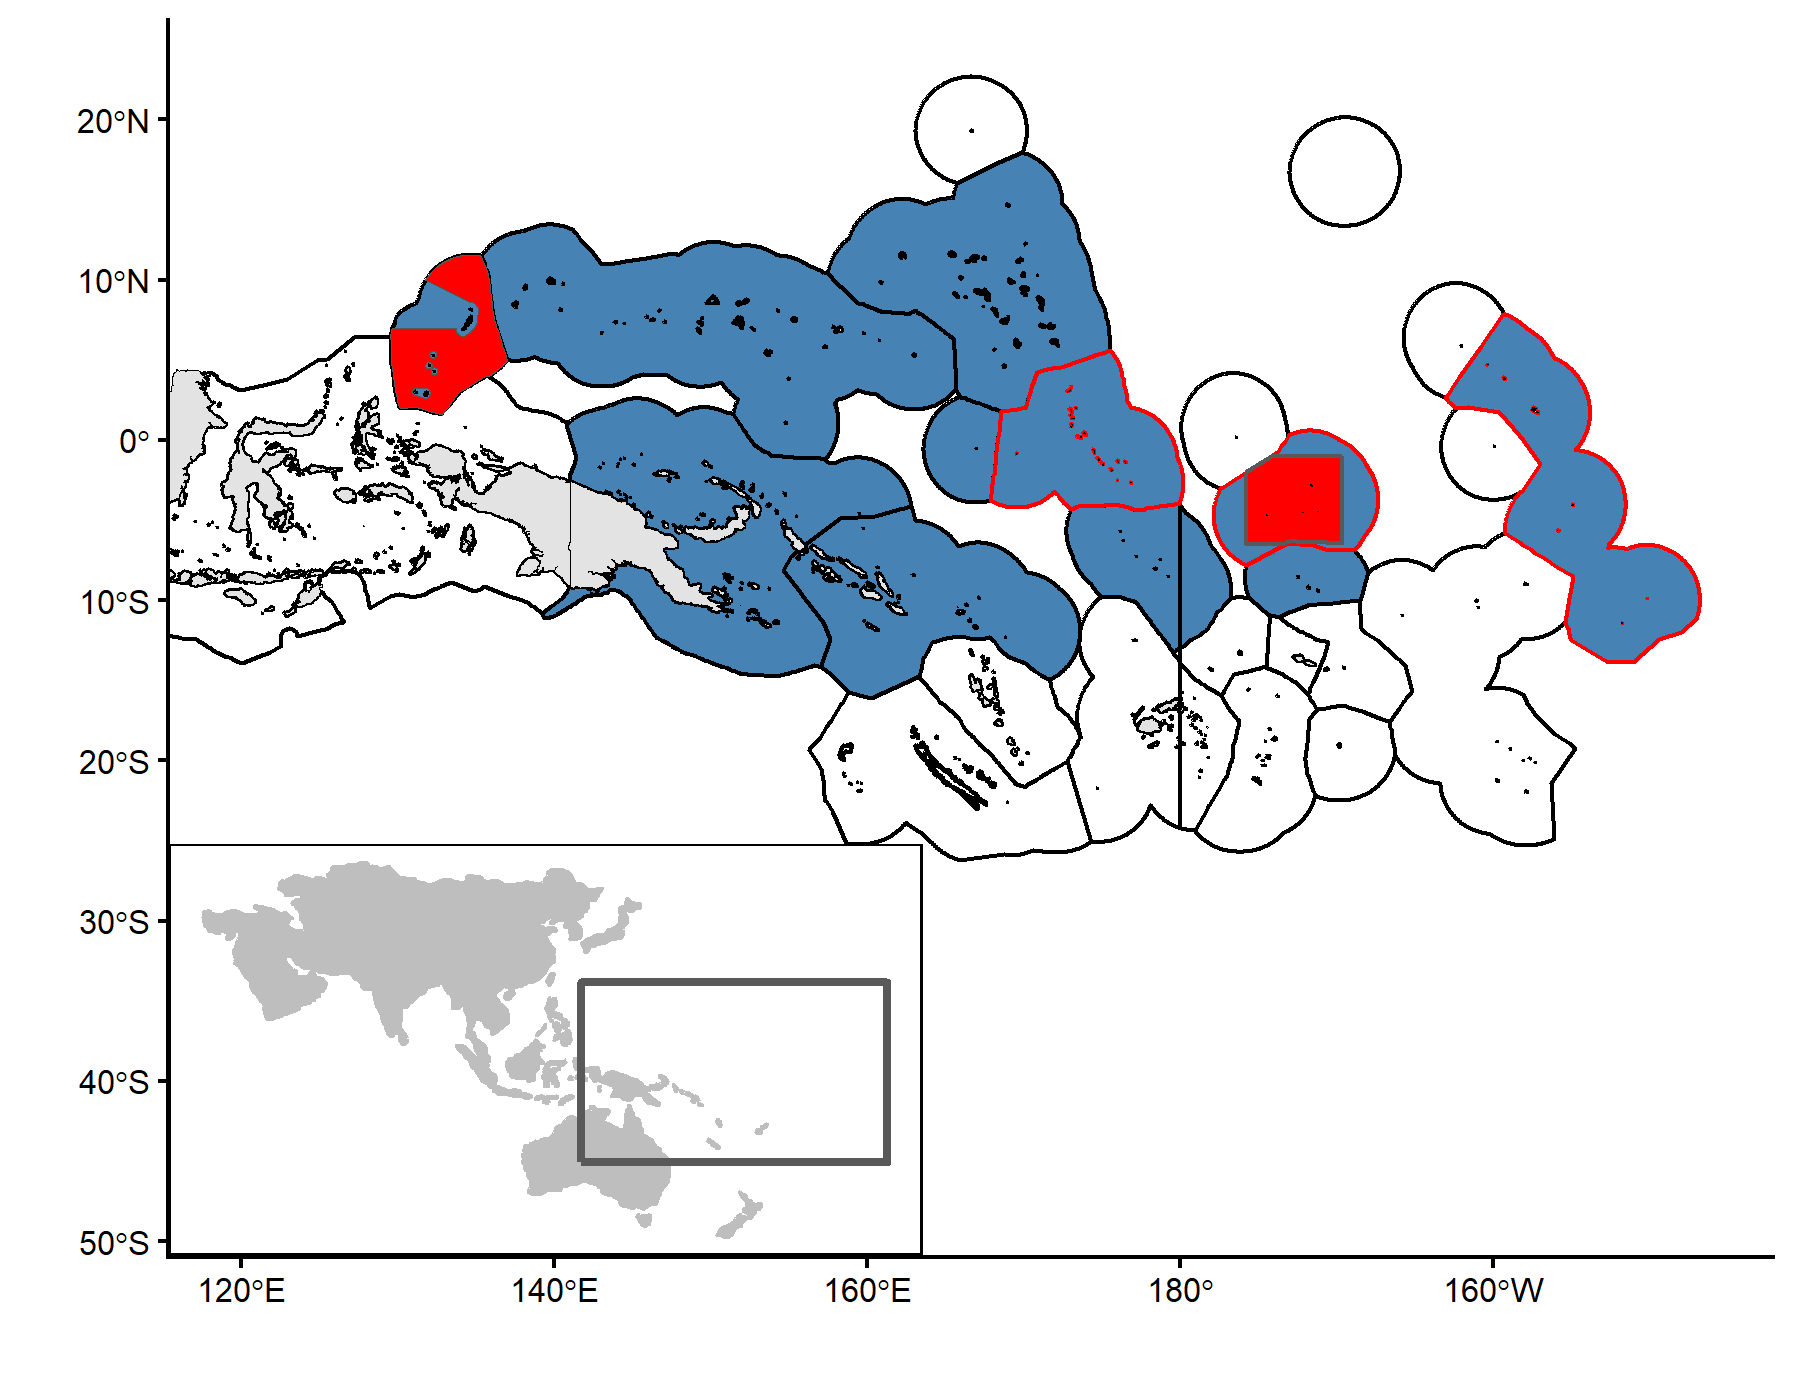
\includegraphics{img/PNA_map.png}
\caption{\label{fig:PNA_map}Map of the Exclusive Economic Zones (EEZs) and Marine Protected Areas in the PNA, the bottom-left inset presents provides a reference for the area. Parties to the Nauru Agreement (PNA) are shown in blue, while empty polygons indicate all others. A red line indicates the Kiribati EEZ. The solid red polygons show The Phoenix Islands Protected Area implemented in 2015 and the proposed Palau National Marine Sanctuary to be implemented in 2020. Land masses are shown in gray. Labels indicate ISO3 country codes for PNA members (PLW: Palau, PNG: Papua New Guinea, FSM: Federal States of Micronesia, SLB: Solomon Islands, NRU: Nauru, MHL: Marshal Islands, KIR: Kiribati, TUV: Tuvalu, TKL: Tokelau).}
\end{figure}

% PNA model output for costs
\begin{figure}[htbp]
\centering
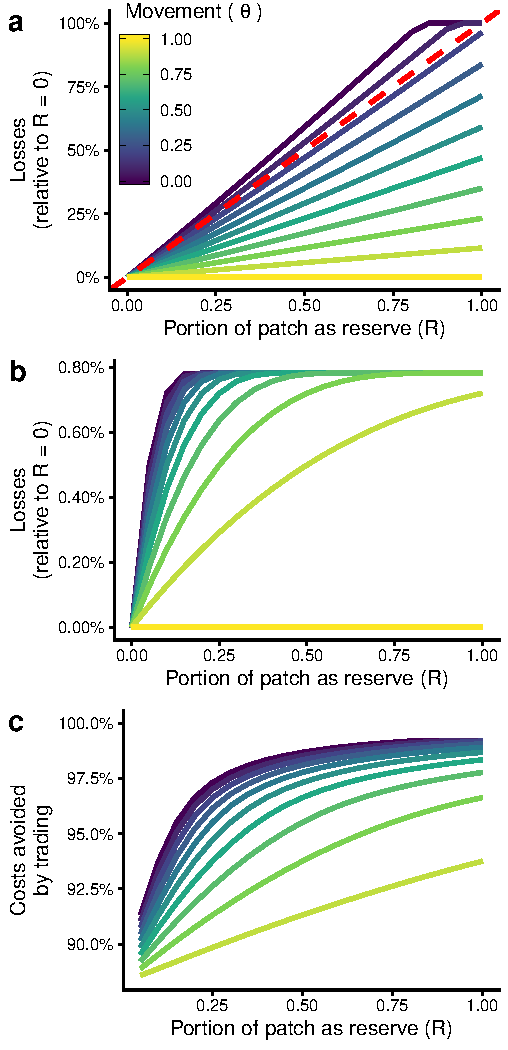
\includegraphics{img/PNA_model.pdf}
\caption{\label{fig:PNA_model}Cost of spatial closures in a vessel-day fishery. Each line represents a possible value of within-country stock movement ($\theta$; line colors), with $\theta = 0$ representing a stock that doesn't move to $\theta = 1$ depicting a stock that continuously moves between the reserve and the fishing zone. The revenue losses to Country 1 (vertical axis) are relative to a fishery with no spatial closures, and are shown as a function of reserve size ($R$; horizontal axis), from no reserve ($R = 0$) to closing the entire Exclusive Economic Zone ($R = 1$). Costs are shown for Country 1 when there is no trading (A) and when trading is allowed (B; note the change in axis limits). Costs avoided by trading are shown in (C). Dashed red line in (A) is a 1:1 line. When trading between countries occurs, 88\% to 99\% of revenue losses can be avoided.}
\end{figure}

% Costs of different allocation rules
\begin{figure}[htbp]
\centering
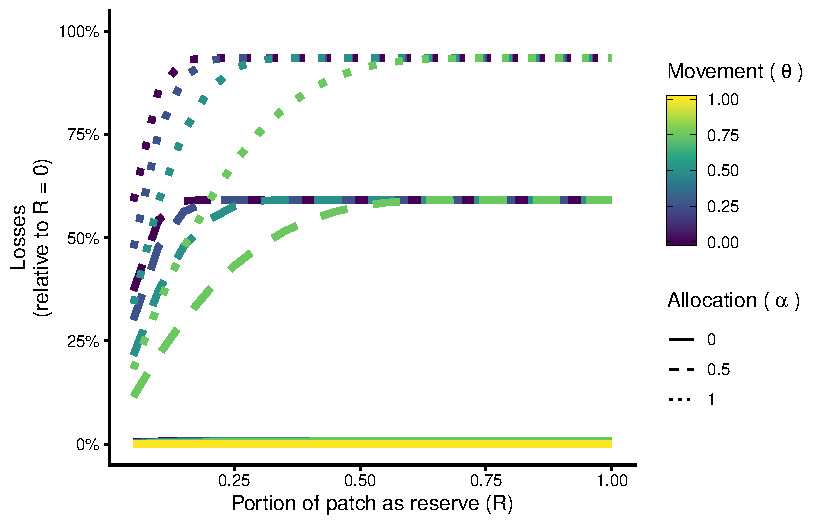
\includegraphics{img/allocation_cost_plot.pdf}
\caption{\label{fig:allocation_cost_plot}Costs of a spatial closure for Country 1 under different allocation rules. Each line represents the revenue losses for a combination of allocation rules ($\alpha$; line type) and movement ($\theta$; color) for different reserve sizes ($R$; horizontal axis). A value of $\alpha = 1$ implies that allocations are based entirely on historical effort, while a value of $\alpha = 0$ implies a 100\% biomass-based allocation rule. A value of $\theta = 0$ represents a stock that doesn't move, and $\theta = 1$ depics a stock that continuously moves between the reserve and the fishing zone. The proportion of the Exclusive Economic Zone closd to fishing is given by $R$. An effort-based allocation and low within-country movement values result in the highest costs. Cost can be minimized for all movement values if allocation is based on biomass within each country’s waters.}
\end{figure}

% Effort redistribution bars for PNA and KIR
\begin{figure}[htbp]
\centering
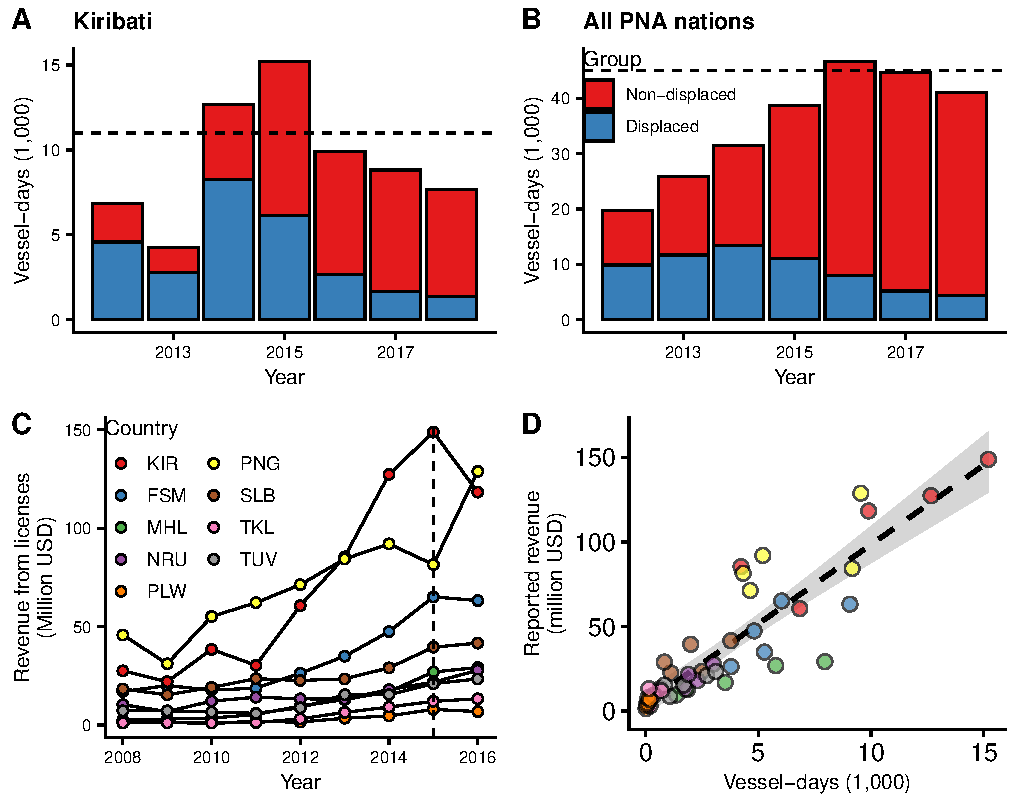
\includegraphics{img/empirical.pdf}
\caption{\label{fig:empirical}Effort displacement and license revenues. Panels (A) and (B) show AIS-derived annual vessel-days for Kiribati and for all Parties to the Nauru Agreement (PNA) by 318 tuna purse seine vessels. Annual effort is broken down by displaced (n = 64) and non-displaced (n = 254) vessels. The dashed horizontal lines represent the total allowable vessel-days in Kiribati (11,000 days \cite{yeeting2018stabilising}) and the PNA (45,000 vessel-days). Panel (C) shows annual revenue from fishing license fees by country and year (2008 - 2016) and panel (D) shows the correspondence between FFA-reported revenues and AIS-derived vessel-day observations (2012 - 2016). The dashed line in panel (D) represents line of best fit, and the shaded area represents the standard error around the regression. Colors in panels (C) and (D) are given by ISO3 country codes for PNA members (PLW: Palau, PNG: Papua New Guinea, FSM: Federal States of Micronesia, SLB: Solomon Islands, NRU: Nauru, MHL: Marshal Islands, KIR: Kiribati, TUV: Tuvalu, TKL: Tokelau).}
\end{figure}

% Redistribution of effort
\begin{figure}
\centering
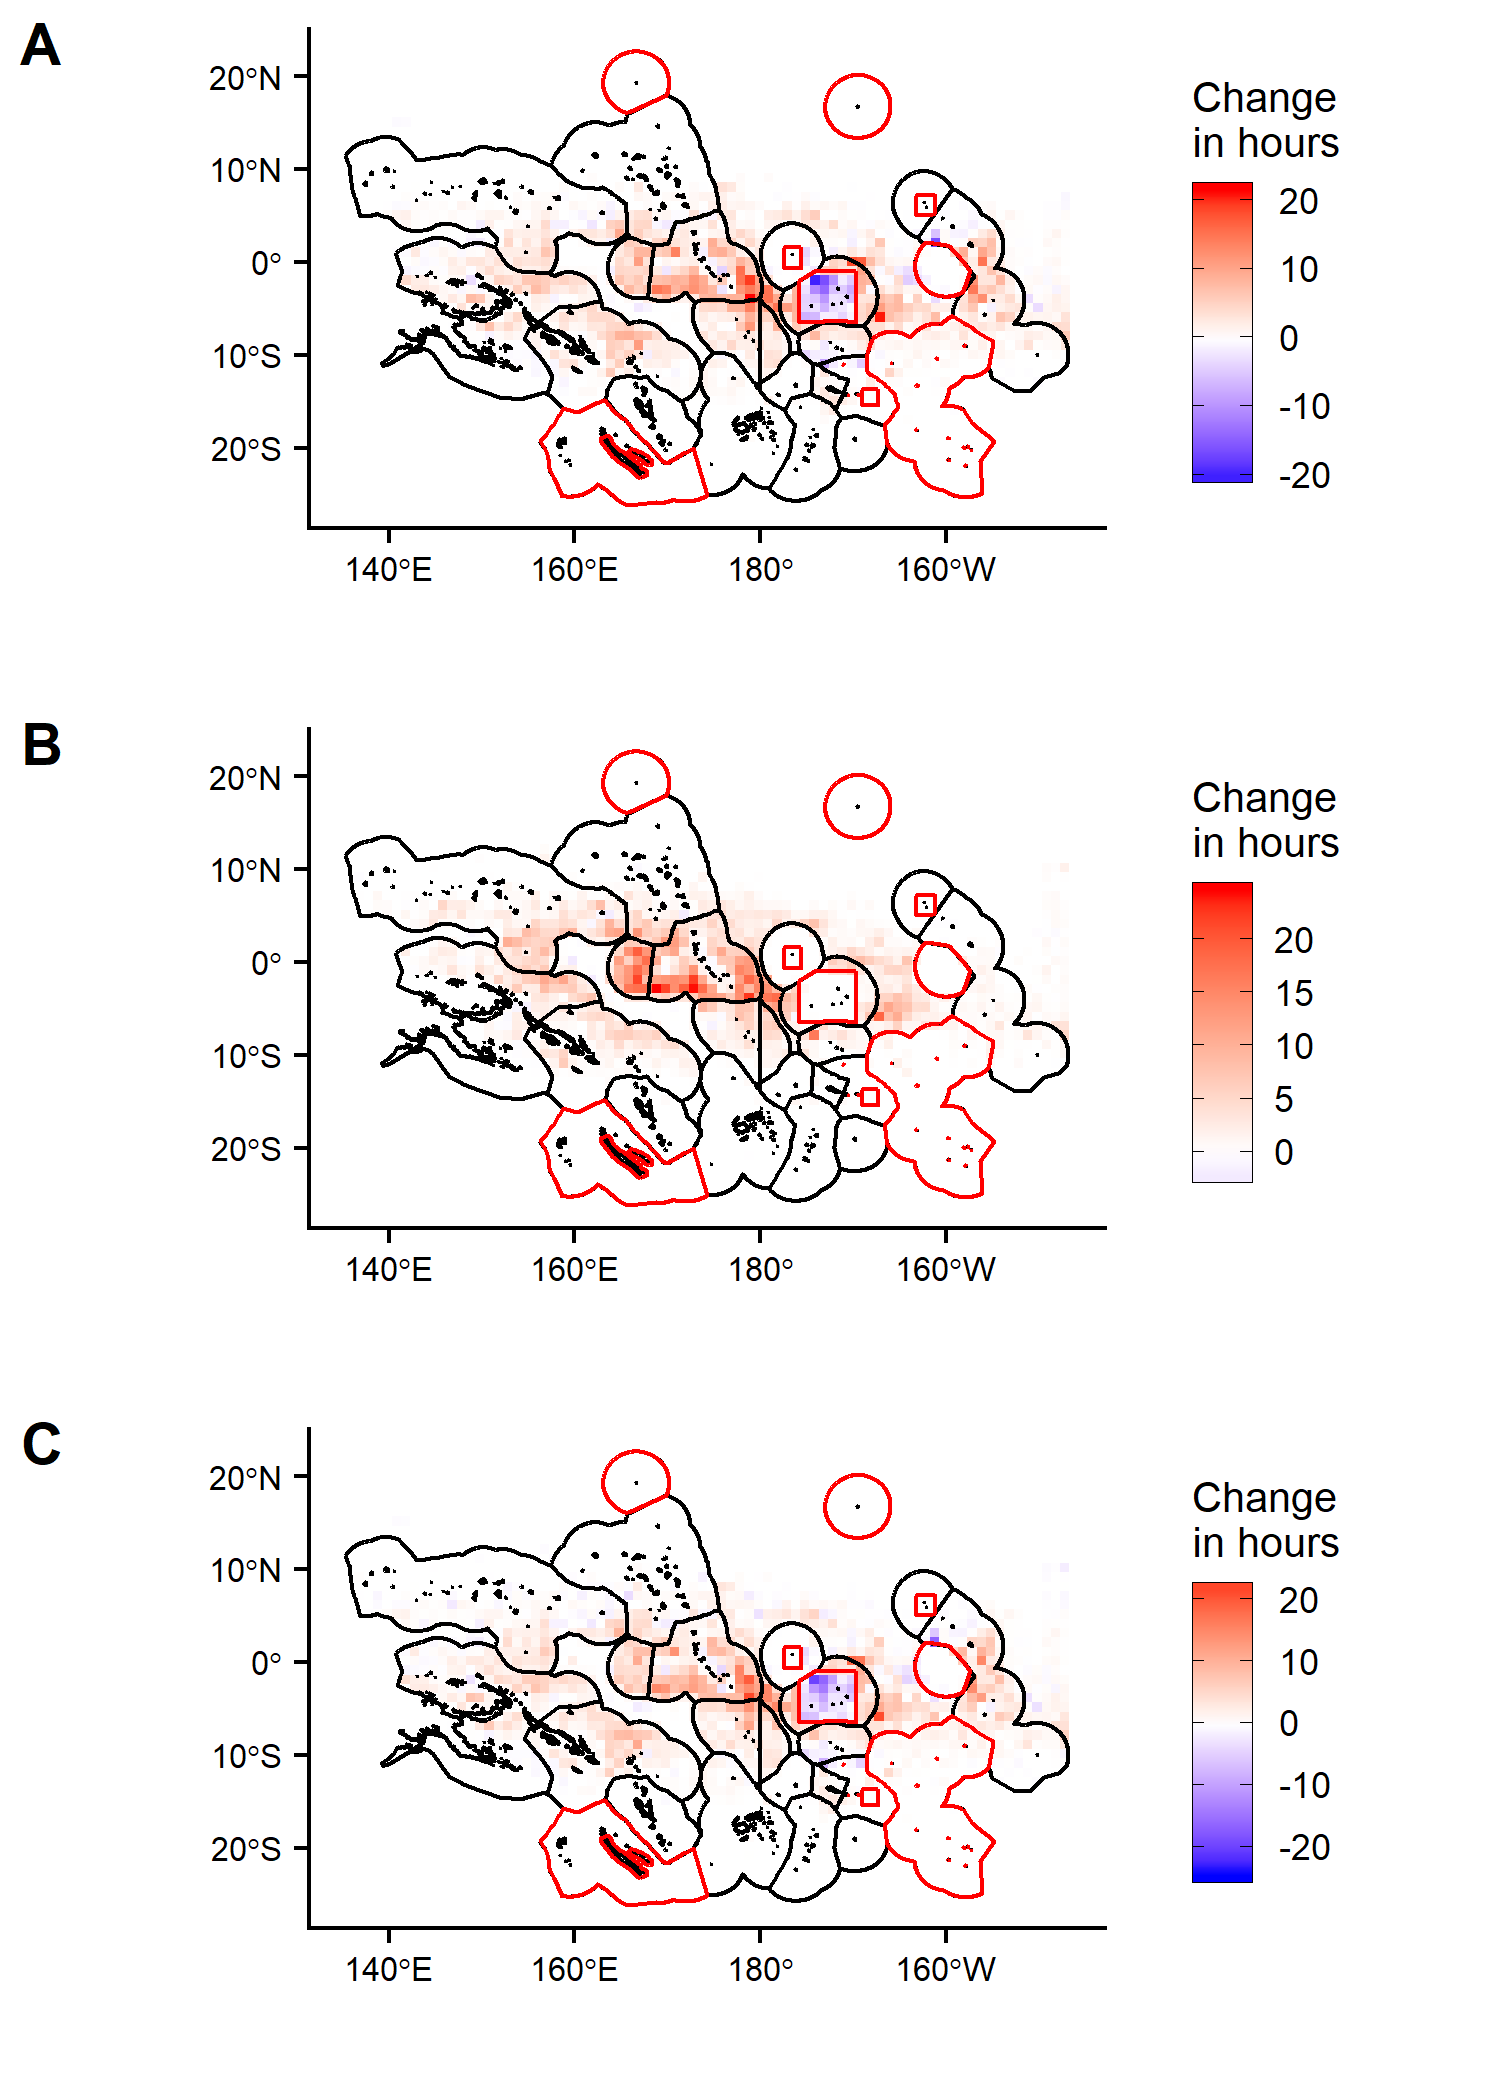
\includegraphics{img/fishing_raster_diff.png}
\caption{\label{fig:fishing_raster_diff}Change in spatial footprint of fishing activity bu 318 tuna purse seines. Black lines show Exclusive Economic Zones (EEZ), red lines show proposed and existing Marine Protected Areas. Panels A and B show the change through time (after - before) for displaced (panel A; n = 64) and non-displaced vessels (panel B; n = 254). Panel C shows the relative difference between A and B (displaced - non-displaced), highlighting areas where displaced vessels redistributed to, relative to non-displaced vessels. Note that displaced vessels allocate more hours to the Gilbert Islands and Line islands EEZs, but also Tuvalu and the high seas surrounding PIPA and Kiribati's EEZ.}
\end{figure}

\end{document}
